\documentclass[3p,twocolumn]{elsarticle}
 
 
 \usepackage{graphicx}%
 \usepackage{multirow}%
 \usepackage{amsmath,amssymb,amsfonts}%
 \usepackage{amsthm}%
 \usepackage{mathrsfs}%
 \usepackage[title]{appendix}%
 \usepackage{xcolor}%
 \usepackage{textcomp}%
 \usepackage{manyfoot}%
 \usepackage{booktabs}%
 \usepackage{algorithm}%
 \usepackage{algorithmicx}%
 \usepackage{algpseudocode}%
 \usepackage{listings}%
 \usepackage{natbib}
 
 \theoremstyle{thmstyleone}%
 \newtheorem{theorem}{Theorem}%  meant for continuous numbers
 %%\newtheorem{theorem}{Theorem}[section]% meant for sectionwise numbers
 %% optional argument [theorem] produces theorem numbering sequence instead of independent numbers for Proposition
 \newtheorem{proposition}[theorem]{Proposition}% 
 %%\newtheorem{proposition}{Proposition}% to get separate numbers for theorem and proposition etc.
 
 \theoremstyle{thmstyletwo}%
 \newtheorem{example}{Example}%
 \newtheorem{remark}{Remark}%
 
 \theoremstyle{thmstylethree}%
 \newtheorem{definition}{Definition}%
 
 \raggedbottom
 %%\unnumbered% uncomment this for unnumbered level heads
 
 
 
 
 
 
 
 
 
  
 \usepackage{float}
 \usepackage{fixltx2e}
 \floatstyle{plaintop}
 \restylefloat{table}
 \usepackage{nohyperref}
 \usepackage{relsize}
 \usepackage{caption}
  \usepackage{amsmath}
 \usepackage{amssymb}

 \usepackage{multirow}
 \usepackage{graphicx}
 \usepackage{caption}
 \usepackage{epstopdf}
 \usepackage{bm}

 \usepackage[numbers]{natbib}
 %\usepackage{natbib}
 \usepackage{xcolor}
 \usepackage{subfigure}
 \usepackage{lscape}
 \usepackage{array}
 \usepackage{threeparttable}
 %\usepackage{ntheorem}
 %\newtheorem{defn}{Definition}
 \usepackage{algorithmicx}
 %\usepackage[boxruled,linesnumbered,ruled,vlined]{algorithm2e}
 \usepackage{latexsym}
 \raggedbottom
 \usepackage{url}
 \tolerance=1
 %%%%%%%%%%%%%%%%%%%%%%%%%%%%%%
 \emergencystretch=\maxdimen
 \hyphenpenalty=10000
 \hbadness=10000
 %%%%%%%%%%%%%%%%%%%%%%%%%%%%%%
 
 
  
 \begin{document}
 
 \begin{frontmatter}
 
 
 \title{Scalable QoS-Aware Cloud Service Composition for Big Data Workflows: A Model-Driven MJAYA Optimization Approach}
 
 
\author[1]{Soumya~Snigdha~Mohapatra} 
\ead{soumyamohapatra@mes.ac.in}
\address[1]{Department of Information Technology, Pillai College of Engineering, Mahatma Education Society, New Panvel, Navi Mumbai, 410206, India}

% Second author
\author[2]{Rakesh Ranjan Kumar}
\ead{rakeshranjan.cdac@gmail.com}
\address[2]{Department of Computer Science and Engineering, C V Raman Global University, Bhubaneswar, 752054, India}

% Third author (Corresponding author)
\author[3]{Abhinav Tomar\corref{cor1}}
\ead{abhinav.tomar@nsut.ac.in}
\address[3]{Department of Computer Science and Engineering, Netaji Subhas University of Technology, New Delhi, 110078, India}

% Corresponding author indication
\cortext[cor1]{Corresponding author: Abhinav Tomar}
 
 \begin{abstract}
 
Cloud Service Composition (CSC) for big data workflows requires selecting concrete services for abstract tasks under multiple Quality of Service (QoS) constraints, resulting in a large-scale NP-hard optimization problem. Many existing CSC solutions rely on metaheuristic algorithms that require careful hyperparameter tuning, which reduces robustness and practical deployability. This study proposes MJAYA, a model-driven, parameter-light optimization algorithm that extends the JAYA framework with adaptive diversity regulation and probabilistic update control to improve exploration–exploitation balance during service selection. The method directly incorporates QoS attributes into the search process and eliminates algorithm-specific parameter calibration. MJAYA is evaluated on synthetic and benchmark workflow datasets against several representative metaheuristic optimizers using standard QoS metrics and nonparametric statistical tests. Results show consistently higher QoS fitness, faster convergence, and lower solution variance across workflow sizes and weight settings. \textcolor{blue}{Sensitivity analysis further confirms stability under varying QoS weight configurations. These findings demonstrate that MJAYA provides a scalable and practically deployable 
optimization framework for QoS-aware cloud service composition in data-intensive and dynamic cloud environments. MJAYA is designed as an offline planning optimizer that can be embedded in a 
service-composition engine as a periodic recomputation module, triggered by QoS profile refreshes or service pool changes.}
 
 \end{abstract}
 \begin{keyword}
Quality of Service (QoS) \sep Cloud Service Composition (CSC) \sep Workflow Optimization \sep Big Data Workflows \sep Computational Efficiency\end{keyword}
 
 \end{frontmatter}
 
 \section{Introduction}
 \label{s1}

Cloud computing is widely recognized as one of the most transformative paradigms in modern information technology due to the substantial benefits it offers in terms of flexibility, scalability, and cost efficiency. By delivering IT-enabled capabilities as elastic and scalable services, cloud computing allows users to access computing resources, platforms, and applications on demand, without the burden of owning, managing, or maintaining the underlying infrastructure 
\cite{Zheng2017qos}. This service-oriented delivery model has led to the proliferation of cloud services with equivalent functionality but varying pricing structures and performance characteristics, collectively referred to as Quality of Service (QoS) attributes. \textcolor{blue}{In this work, the term ``big data workflows'' refers to data-intensive cloud workflows---a standard usage in the cloud service composition literature~\cite{jula2014cloud}---characterised by large combinatorial service pools that make exhaustive composition search computationally infeasible.}

The abundance of functionally similar cloud services presents a significant challenge for consumers, who must identify solutions that best satisfy their functional and non-functional requirements. Since no single service can optimally fulfill all user expectations, selecting an appropriate cloud service often becomes a complex decision-making process, frequently resulting in service dissatisfaction or rejection. Consequently, there is a growing reliance on service composition, particularly in industrial and enterprise domains such as supply chain management, finance, accounting, Science, and multimedia applications, where multiple services must be dynamically integrated to address complex operational requirements.


In practice, major cloud service providers, including Amazon, IBM, Microsoft, and Google, offer a wide range of cloud services that have gained considerable attention due to their ability to deliver reliable, high-performance hardware and software resources at reduced cost, while alleviating concerns related to security management, infrastructure maintenance, and scalability. Moreover, the pay-as-you-go pricing model enables providers to offer services in diverse configurations aligned with customer-defined Service Level Agreements (SLAs).
As the number of available cloud services continues to grow, the service composition problem increasingly manifests as a decision problem involving the selection of component services from a set of alternatives that provide identical functionality but differ in QoS parameters \cite{alrifai2008scalable}. Addressing this challenge requires the effective composition of existing services into a composite service that satisfies user requirements while optimizing QoS constraints, thereby underscoring the importance of robust and scalable QoS-aware service composition mechanisms \cite{eisa2020modelling}. 


For each abstract task in a workflow, multiple concrete services may offer the same functional capabilities but differ in QoS. Therefore, the selection of a concrete service must be guided primarily by QoS considerations. Traditional approaches, such as hybrid Multi-Criteria Decision-Making (MCDM) techniques \cite{kumar2018multi, kumar2018novel, liu2016decision}, have been applied to rank cloud services based on QoS. However, these methods tend to be rigid, focus on selecting a single service, and are often inadequate for real-time or large-scale applications. In practice, multiple compositions may exist to satisfy a business process, with a large and dynamic pool of candidate services. Exhaustively exploring all possible combinations becomes computationally infeasible; for instance, with $m$ abstract services and $n$ candidate services per task, there are $n^m$ possible compositions, rendering the problem NP-hard. Consequently, effective service composition requires optimization approaches that can approximate optimal solutions while meeting both functional and non-functional requirements.


Simulation tools have been developed to implement MCDM models for evaluating cloud services based on QoS attributes, incorporating both subjective and objective measures. However, as user requirements and service offerings become increasingly complex, selecting a single service is often insufficient. Composing multiple services becomes necessary, and variations in QoS—such as response time, availability, and cost—can significantly influence user satisfaction, provider reputation, and revenue.


Meta-heuristic algorithms are well-suited for solving NP-hard problems like cloud service composition \cite{anwit2020tour, anwit2020scheme}. These algorithms explore the search space using stochastic strategies to identify near-optimal solutions. Their effectiveness depends on a careful balance between exploration (searching new regions) and exploitation (refining promising solutions). Insufficient diversity can lead to premature convergence, while excessive diversity may slow convergence. Although numerous enhanced heuristics and meta-heuristics have been proposed to improve solution quality, challenges remain in balancing exploration and exploitation and in tuning algorithmic hyperparameters, which often increases computational complexity. Recent research in cloud and distributed computing optimization increasingly emphasizes hybrid and adaptive metaheuristic frameworks to address multi-objective scheduling and service selection challenges.  For example, a hybrid Cheetah–Dung Beetle Optimization Algorithm has been proposed for cloud–fog job scheduling to balance latency, energy consumption, and cost, demonstrating consistent improvements across real workload traces such as NASA iPSC and HPC2N datasets \cite{gurrala2026novel}. Similarly, multi-objective resource scheduling in IaaS environments has been advanced through hybrid evolutionary–clustering models that integrate NSGA-II with adaptive swarm intelligence, achieving higher resource utilization and lower scheduling overhead under dynamic workloads \cite{radhamani2025multi}. In workflow-oriented cloud environments, adaptive mutation-enhanced snake optimizer variants have shown strong performance for budget-constrained heterogeneous workflow scheduling, significantly reducing makespan while improving feasible-solution discovery rates \cite{zhang2025adaptive}. Beyond scheduling efficiency alone, adaptive trust-aware and policy-driven evaluation frameworks have also been introduced for multi-cloud ecosystems to support reliable service selection under fluctuating QoS and SLA conditions \cite{gupta2025adaptive}. Complementing metaheuristic approaches, multi-criteria decision-making–based service composition models combining AHP and TOPSIS with entropy weighting have demonstrated improved ranking accuracy and bias reduction in large cloud service pools \cite{swathi2025adaptive}. These developments collectively indicate a strong research trend toward adaptive, hybrid, and parameter-light optimization strategies for scalable QoS-aware cloud service selection and composition, which directly motivates the diversity-regulated parameter-light optimization framework proposed in this work.


To address these issues, this paper employs the JAYA optimization algorithm, which is inherently parameter-light and guides the search toward the best solution without requiring additional control parameters. Nevertheless, the original JAYA algorithm exhibits relatively slow convergence in complex service composition scenarios. Even recent comparative studies further demonstrate the effectiveness of metaheuristic and JAYA-family optimization methods in multi-objective engineering optimization, where approaches such as GA, TLBO, and multi-objective JAYA have shown superior parameter tuning and convergence behavior when combined with learning-based models \cite{siyoum2025comparative, chanie2025optimization}. These results reinforce the practical value of parameter-light and hybrid metaheuristic strategies, motivating continued refinement of JAYA-based optimizers for complex multi-criteria search spaces. To overcome the limitation of JAYA in high-dimensional complex search spaces, we propose a modified JAYA (MJAYA) approach that enhances the balance between exploration and exploitation, consistently seeking optimal or near-optimal service compositions. The key contributions of this study are summarized as follows:



\begin{itemize}
	\item A novel enhanced optimization framework, MJAYA, is proposed for QoS-aware cloud service composition, which operates without algorithm-specific hyperparameter tuning and maintains stable performance across multiple datasets.
	
	\item MJAYA incorporates a probabilistic adaptive control mechanism and diversity-guided update strategy that improves convergence behavior and achieves a more effective balance between exploration and exploitation compared to baseline methods.
	
	\item Comprehensive experimental evaluation using standard benchmark workflows and statistical validation tests (including Wilcoxon signed-rank and Quade tests) demonstrates that the proposed optimizer consistently outperforms several well-known metaheuristic algorithms in solution quality and convergence efficiency.
	
	\item The proposed method shows strong scalability across different workflow sizes and candidate service pool configurations, with fast execution suitable for practical cloud service selection scenarios.
\end{itemize}



The remainder of this paper is structured as follows: Section 2 reviews related research on QoS-aware cloud service composition using bio-inspired and meta-heuristic algorithms. Section 3 discusses the modeling of service composition based on QoS characteristics. In Section 4, we formulate the objective function and implement the proposed optimization approach. Section 5 presents the experimental evaluation and results analysis of the proposed method. Finally, Section 6 concludes with key observations.

 \section{Related Work}
 
 Quality of Service (QoS) is widely recognized as a key indicator of non-functional performance requirements for online and cloud services, and it plays a central role in differentiating among functionally similar services \cite{adacal2006mobile, liu2004qos}. Early foundational work summarized the landscape of QoS-driven system design and evaluation, highlighting the importance of performance-oriented service selection and management \cite{menasce2002qos}. To support measurable QoS representation, structured metric models were introduced to quantify different QoS dimensions and enable formal comparison across services \cite{ran2003model}. Community-based service grouping approaches were also proposed to help users address non-functional requirements by organizing services with similar QoS characteristics \cite{perryea2006community}. Later work distinguished between global and local QoS constraints in service-oriented systems, enabling more flexible constraint modeling in composite applications \cite{ardagna2005global}. Middleware frameworks for QoS-aware service composition were subsequently developed to support constraint-driven service selection and aggregation, where linear QoS models were used as a basis for global optimization criteria \cite{zeng2004qos}. These approaches collectively emphasize precise QoS measurement and structured evaluation models as the foundation for QoS-aware decision-making.

Cloud service selection can also be formulated as a Multi-Criteria Decision Making (MCDM) problem, where candidate services are evaluated across multiple QoS attributes simultaneously \cite{youssef2020integrated, kumar2021ccs}. However, classical multi-criteria programming models are often too rigid for real cloud environments. Two major challenges arise in practice. First, many QoS attributes are uncertain or dynamically varying due to heterogeneous infrastructure, changing configurations, and fluctuating network conditions, which makes precise value specification difficult. Second, the relative importance (weights) of QoS criteria is often derived from human judgment and may therefore be imprecise or subjective. Broker-based selection strategies were introduced to partially address these limitations by mediating between users and providers using QoS-aware matching mechanisms \cite{d2008qos}. Nevertheless, uncertainty handling remains a critical concern, and fuzzy modeling has emerged as an effective way to represent imprecise QoS values and linguistic preferences.

In recent years, fuzzy set theory and fuzzy decision-making frameworks have been widely applied to online and cloud service selection problems to better capture uncertainty and subjective evaluation \cite{bagga2019qos}. Fuzzy Multi-Criteria Decision Making (FMCDM) methods have been used to model user preferences more realistically and to support service ranking under ambiguity \cite{chen2003fuzzy}. Hybrid weighting strategies combining subjective and objective components have also been proposed, where human preference determines subjective weights and entropy-based measures derive objective weights to improve evaluation reliability \cite{xiong2007qos}. These approaches introduce synthetic weighting schemes to balance both perspectives. However, much of this work primarily focuses on selecting a single best service. In contrast, cloud service composition requires building an integrated service execution model and selecting optimal combinations of services that collectively satisfy end-to-end QoS requirements, which introduces additional optimization and dependency challenges \cite{yu2005service}.There are a few fundamental system aspects that must be taken into account since cloud services are dynamic:
 
 \begin{itemize}
 	\item A broad and dynamic group of candidate services may be available to fulfill a particular capability.
 	\item Instead of focusing just on any one service component, the quality of a composite service is evaluated from beginning to end. Additionally, each individual service component decides together on the overall quality.
 	\item There could be several different methods to complete a business process for a composite Web service.
 	\item A business process component services could continue to develop. The worldwide system variances, such as service outages and upgrades, must also be accommodated by a business process.
 \end{itemize}
 
 \begin{table*}[!t]
 	\centering
 	\caption{Summary of related works in comparison with the proposed approach.}
 	\label{tab:QOS1}
 	\scalebox{0.62}{
 		\begin{tabular}{llllllc}
 			\hline\\\textbf{Reference} &  \textbf{Techniques} &  \textbf{Objective}   &  \textbf{Research Gap}  
 			\\ \hline\\
 			Dahan et al.~\cite{dahan2021enhanced} & \begin{tabular}[c]{@{}l@{}}  Ant Colony Optimization(ACO),\\ Genetic Algorithm(GA) \end{tabular} &\begin{tabular}[c]{@{}l@{}}Composite Service Selection\\Avoid stagnation problem,\\Enhance performance   \end{tabular} &\begin{tabular}[c]{@{}l@{}} G1/G2  \end{tabular}        \\\\
 			
 			Gavvala et al.~\cite{gavvala2019qos} & \begin{tabular}[c]{@{}l@{}}  Eagle strategy with Whale Optimization \\Approach (ESWOA)\end{tabular} &\begin{tabular}[c]{@{}l@{}}Composite Service Selection\\Reduced randomness\\ Improved convergence rate \end{tabular} &\begin{tabular}[c]{@{}l@{}}G2 due to more hyper-parameters\\G9  \end{tabular}        \\\\
 			
 			Haytamy and Omara~\cite{haytamy2020deep} & \begin{tabular}[c]{@{}l@{}}  Long Term Short Term Memory(LSTM) \\ with PSO\end{tabular} &\begin{tabular}[c]{@{}l@{}}Cloud Service Composition \\Capture non-linear correlations\\ among QoS attributes  \end{tabular} &\begin{tabular}[c]{@{}l@{}}G1,G2 \end{tabular}        \\\\
 			Youssef et al.~\cite{youssef2020integrated} & \begin{tabular}[c]{@{}l@{}}  MCDM approach with TOPSIS \\ + Best Worst Method(BWM) \end{tabular} &\begin{tabular}[c]{@{}l@{}}Service Selection and Ranking\\Less Computational Complexity \end{tabular} &\begin{tabular}[c]{@{}l@{}}G3,G4  \end{tabular}           \\\\
 			Khanam et al.~\cite{khanam2018qos} & \begin{tabular}[c]{@{}l@{}} PSO with optimal set of concrete \\services \end{tabular} &\begin{tabular}[c]{@{}l@{}}Composite Service Selection \\Improved convergence rate\\than PSO \end{tabular} &\begin{tabular}[c]{@{}l@{}}G1 due to random search strategy  \end{tabular}            \\\\
 			Naseri and Navimipour~\cite{naseri2019new} & \begin{tabular}[c]{@{}l@{}}  Agent Based Method \\ with PSO\end{tabular} &\begin{tabular}[c]{@{}l@{}}Composite Service Selection\\Improved Performance,\\Reduced waiting time \end{tabular} &\begin{tabular}[c]{@{}l@{}}G5 where distribution factor \\ of importance is significant  \end{tabular}         \\\\
 			Kumar et al.~\cite{kumar2018novel} & \begin{tabular}[c]{@{}l@{}} MCDM approach AHP Based SaaS \\ Selection + TOPSIS for ranking  between\\ cloud services\end{tabular} &\begin{tabular}[c]{@{}l@{}}Service Selection and Ranking\\Simple assessment model \end{tabular} &\begin{tabular}[c]{@{}l@{}} G4,G6,G7\end{tabular}           \\\\
 			Jatoth et.al~\cite{jatoth2019optimal} & \begin{tabular}[c]{@{}l@{}}  Adaptive genotype  and evolution\\ based GA\end{tabular} &\begin{tabular}[c]{@{}l@{}}Composite Service Selection\\Considers connectivity constraints\\ between QoS parameters\end{tabular}  &\begin{tabular}[c]{@{}l@{}}G8  \end{tabular}        \\\\
 			
 			Kumar et al.~\cite{kumar2021ccs} & \begin{tabular}[c]{@{}l@{}} MCDM approach with BWM and \\TOPSIS \end{tabular} & \begin{tabular}[c]{@{}l@{}}\\ Service Selection and ranking\\Less computational complexity \\than AHP  \end{tabular}  & \begin{tabular}[c]{@{}l@{}} G3,G4,G9 \end{tabular}       \\\\
 			
 			Eisa et al.~\cite{eisa2020modelling} & \begin{tabular}[c]{@{}l@{}} MCDM approach with AHP and \\Simple Additive Weighting(SAW)  \end{tabular} & \begin{tabular}[c]{@{}l@{}}\\ Service Selection and ranking\\Considers Multi-level QoS attributes\\Ensures credibility \\  \end{tabular}  & \begin{tabular}[c]{@{}l@{}} G4 \end{tabular}       \\\\
 			
 			
 			Proposed approach & \begin{tabular}[c]{@{}l@{}} Modified JAYA optimization\\conditional probabilistic adaptive control Validation\\Wilcoxon Signed Rank Test\\Quade Test \end{tabular} & \begin{tabular}[c]{@{}l@{}}\\ QoS aware Composite Service Selection\\ Faster convergence\\Less hyperparameters\\Less computational complexity\\More consistent and robust  \end{tabular}  & \begin{tabular}[c]{@{}l@{}} Can expand our work\\by transfer learning's ability \\to scale  massive datasets, \\so that we may investigate\\ every possible QoS metric. \end{tabular}       \\\\
 			\hline
 	\end{tabular}}
 	\begin{tablenotes}
 		\small
 		\item \textit{\textbf{G1}: May result in higher execution time and increase in time complexity; \textbf{G2}: More computational complexity; \textbf{G3}: Can be improved with the multi-cloud environment; \textbf{G4}: Increase in a number of criteria  may result in an increase in computational complexity, strenuous implementation; \textbf{G5}: Utilisation of data center percentage is less; \textbf{G6}: Matrix-based multilevel laborious comparisons; \textbf{G7}: Limitation of AHP due to pairwise comparison; \textbf{G8}: With the increase in candidate service can result in an increase in search space, slow convergence, stuck in local optima; \textbf{G9}: Interrelationships among criteria have not considered.  } 
 	\end{tablenotes}
 \end{table*}
During the service composition process, a large number of feasible candidate combinations may be generated, and evaluating all possibilities leads to exponential computational complexity. Specifically, if a workflow contains $m$ abstract services and each has $n$ candidate concrete services, then up to $n^m$ distinct compositions are possible \cite{priya2021cloud}. Since this problem is NP-hard, exact optimization is computationally impractical for realistic workflow sizes. Therefore, the objective is to identify near-optimal cooperative solutions that satisfy both functional requirements and non-functional QoS constraints, which naturally formulates the problem as a large-scale optimization task.

To obtain near-global optimal solutions, researchers have widely adopted meta-heuristic optimization algorithms inspired by biological evolution and natural phenomena, including swarm intelligence and collective animal behavior models \cite{asghari2018nature}. These approaches have demonstrated strong performance on complex combinatorial optimization problems. In the context of QoS-aware cloud service composition, several Particle Swarm Optimization (PSO)-based methods have been proposed \cite{zhang2014qos, khanam2018qos, tomar2022decision, naseri2019new}. Hybrid variants have also been developed to improve search performance, such as PSO combined with Genetic Algorithms \cite{faruk2016genetic} and PSO integrated with discrete immune optimization to escape local minima \cite{zhao2012improved}. Ant Colony Optimization techniques have likewise shown effectiveness for QoS-aware composition problems \cite{dahan2021enhanced}. More recently, learning-based approaches such as Long Short-Term Memory (LSTM) models have also been explored to support optimization and prediction in service selection scenarios \cite{haytamy2020deep}. Comprehensive surveys provide detailed overviews of candidate service representation, fitness evaluation models, and evolutionary operator design in cloud composition literature \cite{da2020survey, jula2014cloud}.

Despite their strengths, existing metaheuristic approaches exhibit inherent limitations related to population diversity control and convergence behavior. Effective search requires a careful balance between exploration and exploitation within the evolving solution population. Insufficient diversity can lead to premature convergence when local exploitation dominates, reducing the likelihood of discovering globally competitive solutions. Conversely, excessive diversity may support broader exploration but often slows convergence rates \cite{youssef2020integrated}. Maintaining a balanced search dynamic is therefore essential for reliable optimization performance. To address this, several hybrid strategies have been introduced, including Eagle strategy variants incorporating Lévy flight and firefly-based search mechanisms \cite{asghari2018nature, gavvala2019qos}. Evolutionary GA-based composition models have also been proposed to handle multiple QoS parameters and service connectivity constraints within composite workflows \cite{jatoth2019optimal}.

A comparative summary of cloud service selection approaches based on metaheuristics, MCDM models, and non-MCDM techniques is presented in Table \ref{tab:QOS1}, where research gaps and improvement opportunities are identified as $G_i$ ($i$ = 1 to 9). For example, repeated per-ant per-service updates in ant colony approaches may increase computational overhead ($G_1$, $G_2$) \cite{dahan2021enhanced}, while improper parameter tuning in hybrid swarm strategies can reduce robustness ($G_2$, $G_9$) \cite{gavvala2019qos}. MCDM-based selection methods improve decision structure but may struggle with scalability and dynamic adaptation ($G_3$, $G_4$, $G_6$, $G_7$, $G_9$) \cite{youssef2020integrated, kumar2018novel, kumar2021ccs, eisa2020modelling}. Several PSO- and GA-based methods may also experience premature or slow convergence due to highly non-linear search dynamics \cite{haytamy2020deep, khanam2018qos, naseri2019new, jatoth2019optimal}. In contrast, JAYA-based optimization frameworks reduce sensitivity to parameter tuning while maintaining a structured best–worst guided search process. Diversity-enhanced JAYA variants further improve convergence stability by preserving population spread and strengthening exploration–exploitation balance.
 
\section{Cloud Service Composition Models and QoS}

The key concepts essential for understanding the composite cloud service framework includes the roles of tasks, candidate services, and service composition. Such definitions are presented further:

\textbf{Task} A composite cloud service's fundamental building block is a task. Each task completes a candidate service that executes the component function associated with it. All of the component functions that were successfully accomplished by tasks combine to form the combined functions of the composite service that users selected.

\textbf{Candidate service} The nonfunctional qualities (QoSs) of the candidate service come in a variety of values and are offered by various service providers. All candidate services associated with the same job, albeit having different QoSs, can fulfill the relevant component function of this work.

\textbf{Service composition} It is made up of potential services that are drawn from several jobs. With the aid of a service composition, a specific composite function that the user has defined may be completed and whose QoS attribute is established by the component candidate services.
\begin{figure*}
	\centering
	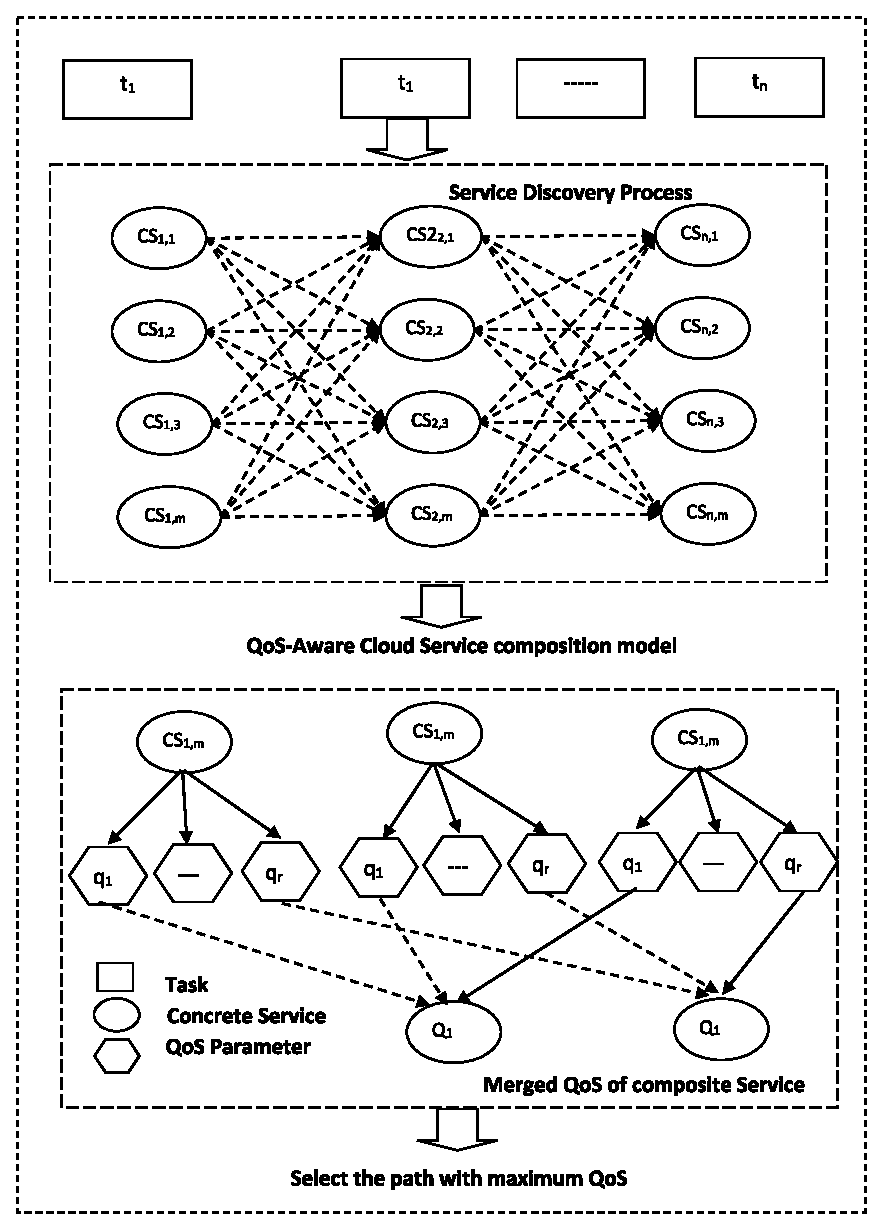
\includegraphics[width=0.7\textwidth]{figures/Final-_2_.eps}
	\caption{Workflow Simulation}
	\label{fig:workflow}
\end{figure*}


The workflow simulation framework illustrated in Figure \ref{fig:workflow} represents the end-to-end QoS-aware cloud service composition pipeline. The model begins with a user-defined workflow consisting of multiple abstract tasks. Each abstract task is mapped to a candidate service pool containing functionally equivalent cloud services with heterogeneous QoS attributes such as response time, availability, cost, and reliability. In the figure, $t_n$ represents a task which is associated with a candidate cloud service $CS_{n,m}$, where $n$ and $m$ represents the $n^{th}$ candidate cloud service and the number of cloud services for $n^{th}$ candidate, respectively. $q_r$ represents the QoS parameter, where $r$ is the number of QoS parameter. During the service discovery process, complex user requirements are typically decomposed into multiple abstract tasks. Each task can be realized by a set of candidate services that provide equivalent functionality but exhibit different QoS characteristics. Consequently, the evaluation and comparison of QoS attributes among candidate services becomes a crucial and challenging problem, as it directly affects the selection of the most appropriate service for each task.

\begin{figure*}
	\centering
	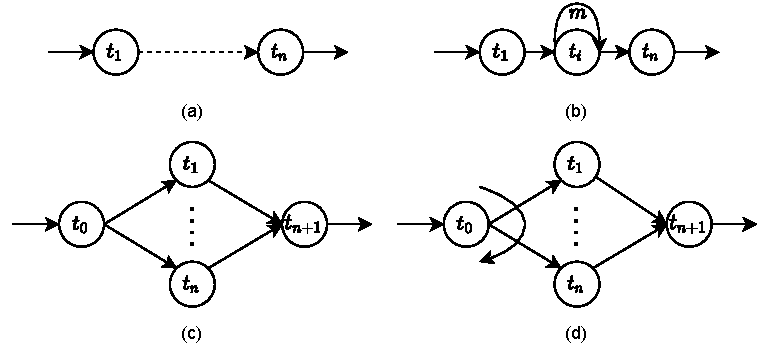
\includegraphics[width=1\textwidth]{figures/11}
	\caption{Service composition models: (a) Sequential (b) Cycle (c) Parallel (d) Branch}
	\label{fig:web_service_model}
\end{figure*}

\subsection{Cloud Service Composition Models}

Cloud service has four basic models as shown in Figure \ref{fig:web_service_model}.
\begin{itemize}
	\item \textbf{Sequential:} In this model, the sequential order of tasks are executed. 
	\item \textbf{Cycle:} A job will be carried out several times in this model.
	\item \textbf{Parallel:} This model allows for simultaneous execution of all parallel activities, but it is unable to go on to the next job until all parallel tasks have been completed.
	\item \textbf{Branch:} With this method, each task in the branch can finish the same component function before going on to the next task when the previous one is finished.
\end{itemize}

It is clear how the parallel and branch structures differ from one another. For the parallel structure, all of the parallel tasks $t_1$ to $t_n$ must be finished in order to go on to task $t_{n+1}$ from task $t_0$. You will move on to task $t_{n+1}$ for the branch structure from task $t_0$ if just one of the tasks $t_1$ to $t_n$ has been finished. \textcolor{blue}{It is important to note that task-level data dependencies and execution-order constraints are defined at the workflow specification layer and are fixed prior to optimization. MJAYA operates at the service selection layer, receiving the fully specified workflow as input and selecting the optimal concrete service for each abstract task---consistent with the standard CSC formulation in~\cite{zeng2004qos, 
jatoth2019optimal}.}

\subsection{QoS Representation}

\textbf{QOS} Four non-functional characteristics of a cloud service are represented by the acronym QOS: cost ($C$), availability ($A$), time ($T$), and reliability ($R$).

Since a composite cloud service is composed of the four core structures outlined above, it is possible to determine the QoSs of a particular service composition using the QoS of those structures. These structures' non-functional characteristics can be determined using the following formulae. By the way, the normalized findings for the non-functional qualities (C, A, T, and R) are computed and shown in Table \ref{tab:QOS}, Equation \ref{eq:pos_norm}, and Equation \ref{eq:neg_norm}.


\begin{table*}[htbp!]
	\caption{QoS functions for various cloud service composition models}
	\label{tab:QOS}
	\centering
	
	\begin{tabular}{@{}lllll@{}}
		\toprule
		\textbf{Service models} & \textbf{Cost} & \textbf{Availability} & \textbf{Time} & \textbf{Reliability} \\ \midrule \\
		\textbf{Sequential}     &   \multicolumn{1}{c}{$\sum_{i=1}^{n} C_i$}    &       \multicolumn{1}{c}{$\prod_{i=1}^{n} A_i$}   &     \multicolumn{1}{c}{$\sum_{i=1}^{n} T_i$}  &       \multicolumn{1}{c}{$\prod_{i=1}^{n} R_i$}    \\\\
		\textbf{Cycle}          &   \multicolumn{1}{c}{$\sum_{i=1}^{n} C_i$}    &       \multicolumn{1}{c}{$\prod_{i=1}^{n} A_i$}   &     \multicolumn{1}{c}{$\sum_{i=1}^{n} T_i$}  &       \multicolumn{1}{c}{$\prod_{i=1}^{n} R_i$}    \\\\
		\textbf{Parallel}       &   \multicolumn{1}{c}{$\sum_{i=1}^{n} C_i$}    &       \multicolumn{1}{c}{$min(A_i)$}              &     \multicolumn{1}{c}{$max(T_i)$}            &       \multicolumn{1}{c}{$\prod_{i=1}^{n} R_i$}     \\\\
		\textbf{Branch}         &   \multicolumn{1}{c}{$min(C_i)$}              &       \multicolumn{1}{c}{$max(A_i)$}              &     \multicolumn{1}{c}{$min(T_i)$}            &       \multicolumn{1}{c}{$max(R_i)$}               \\\\ \bottomrule
	\end{tabular}
\end{table*}

Aspect values must be normalized to the same scale in order to prevent incorrect assessments caused by the multiple measurement metrics of QoS characteristics. Both positive and negative numerical QoS qualities exist. Greater values for positive attributes, such as availability and dependability, suggest higher quality; these values are normalized as in Equation \ref{eq:pos_norm}. Cost and response time are two negative attributes that have the opposite impact when normalized, as shown in Equation \ref{eq:neg_norm}.

\begin{equation}
\hat{Q}=
\begin{cases}
\frac{Q_i-Q_i^{min}}{Q_i^{max}-Q_i^{min}} & Q_i^{max}-Q_i^{min} \neq 0\\    
\hspace{0.8cm}1 &    Q_i^{max}-Q_i^{min} = 0
\end{cases}
\label{eq:pos_norm}
\end{equation}

\begin{equation}
\hat{Q}=
\begin{cases}
\frac{Q_i^{max}-Q_i}{Q_i^{max}-Q_i^{min}} & Q_i^{max}-Q_i^{min} \neq 0\\    
\hspace{0.8cm}1 &    Q_i^{max}-Q_i^{min} = 0
\end{cases}
\label{eq:neg_norm}
\end{equation}

where $Q_i$ and $\hat{Q}_i$ refer to the attribute values of a service before and after normalization, and $Q^{max}_i$ and $Q^{min}_i$ are the maximum and minimum attribute values among all qualifying services, respectively. It is clear that whether a service has positive or negative characteristics, the normalized values lie in the range 0 to 1, $\hat{Q}_i$ $\in$ $[0, 1]$.

\section{Proposed Cloud Service QoS Optimization}

\subsection{Objective Formulation}

The product of each normalized attribute value and its related weight, as illustrated in the normalization equations shown in Equation \ref{eq:pos_norm} and Equation \ref{eq:neg_norm}, can be used to bring all QoS values to a common reference frame that evenly determine the QoS performance of any qualifying service.

This work uses weighted sum modeling as a consistent QoS performance assessment model regardless of their units and ranges to evaluate the multi-dimensional performance of aggregated QoS attribute values. In order to create a weighted summation optimization model, the QoS-driven cloud service composition is then changed as shown in Equation \ref{eq:QoS}. 

\begin{equation}
max(QoS)=\sum_{i=1}^{m} w_i ~ \hat{Q}_i
\label{eq:QoS}
\end{equation}

The sum of weights must be 1, which is a constraint for this objective function as shown in Equation \ref{eq:Con}.

\begin{equation}
\sum_{i=1}^{m}w_i=1
\label{eq:Con}
\end{equation}

where $m$ represents the number of QoS attributes and $w_i$ is the corresponding weight for the $i^{th}$ QoS attribute. In the present research $m$ is considered as 4. $\hat{Q}$ is the normalized QoS attribute as shown in Equation \ref{eq:pos_norm} and Equation \ref{eq:neg_norm}, and QoS attributes are computed using equations in the Table \ref{tab:QOS}.

However, in our present experiment the sequential cloud service composition  model is selected as shown in (Figure \ref{fig:web_service_model}(a)). The objective for the sequential model can be represented as in Equation \ref{eq:obj}.

\begin{equation*}
QoS = \sum_{i=1}^{4} w_i ~ \hat{Q}_i =
\label{eq:obj}
\end{equation*}
\begin{equation}
w_1~\sum_{i=1}^{n} \hat{C}_i + w_2~\prod_{i=1}^{n} \hat{A}_i + w_3~\sum_{i=1}^{n} \hat{T}_i + w_4~\prod_{i=1}^{n} \hat{R}_i
\label{eq:obj}
\end{equation}


where $\hat{A}$ and $\hat{R}$ are the normalized availability and reliability QoS values computed using Equation \ref{eq:pos_norm}. Similarly, $\hat{C}$ and $\hat{T}$ are the normalized cost and time QoS values computed using Equation \ref{eq:neg_norm}. \textcolor{blue}{It is worth noting that the response time ($T$) and cost ($C$) dimensions in the QoS objective directly capture 
service-level execution latency and resource cost---the primary deployment-relevant factors observable from QoS profiles---consistent with the modeling approach in~\cite{zeng2004qos, 
eisa2020modelling}. Infrastructure-level factors such as cross-service communication overhead and instance startup latency require live testbed or simulation experiments and are identified 
as a future validation direction.}

The composite cloud service with the highest assessment score has a greater quality than others since each attribute value has been standardized. When a threshold is present, a service is chosen as soon as its assessment score exceeds the necessary level. If no service meets that criterion, the service requester's needs cannot be met by any service in the repository.

Optimization of the objective function defined in Equation \ref{eq:QoS} 
and Equation \ref{eq:obj} is carried out using the JAYA approach which 
is described further. \textcolor{blue}{It is worth noting that the 
weighted-sum formulation adopted here represents a preference-scalarized, 
single-policy design choice, where the weights $w_i$ encode the 
decision maker's explicit QoS priorities. This is consistent with 
established CSC literature~\cite{jatoth2019optimal, gavvala2019qos, 
haytamy2020deep, eisa2020modelling}. Extension to a Pareto-front 
multi-objective formulation is identified as a future research direction.}


Optimization of the objective function defined in Equation \ref{eq:QoS} and Equation \ref{eq:obj} is carried out using the JAYA approach which is described further. \textcolor{blue}{It is worth noting that the weighted-sum formulation adopted here represents a preference-scalarized, single-policy design choice, where the weights $w_i$ encode the decision maker's explicit QoS priorities. This is consistent with established CSC literature~\cite{jatoth2019optimal, gavvala2019qos, 
haytamy2020deep, eisa2020modelling}. MJAYA is therefore designed as an offline planning optimizer, where the composition plan is computed from available QoS profiles and recomputed when service 
conditions change significantly. Extension to a Pareto-front multi-objective formulation is identified as a future research direction.}

\subsection{Jaya optimization}

Rao \cite{rao2016jaya} recently presented the Jaya algorithm, which is gaining popularity because of how straightforward and reliable it is. With no additional algorithmic hyper-parameters like other algorithms, the current solution in this method always strives to advance toward the best solution.

Assume that the goal function, $f(x)$, is what has to be reduced or maximized. In each iteration $i$, it is assumed that there are $m$ design variables and $n$ potential solutions (i.e., population size $k$=1,2,..,$n$). Let's say that $f(x)_b$ represents the candidates with the best cost for $f(x)$, and $f(x)_w$ represents the candidates with the worst costs among all of the candidates. If $X_{j,k,i}$ represents the value of the $jth$ variable for the $k^{th}$ candidate during the $i^{th}$ iteration, then the equation used to update $X_{j,k,i}$ to $X'_{j,k,i}$ is expressed as in Eq. \ref{jaya1},\ref{jaya2}.


\begin{eqnarray}
\label{jaya1}
\ X'_{j,k,i} = X_{j,k,i} + \Delta X  \\
\label{jaya2}
\Delta X = r^1_{j,i} (X_{j,b,i} -  \lvert X_{j,k,i} \rvert) - r^2_{j,i} (X_{j,w,i} -  \lvert X_{j,k,i} \rvert)
\end{eqnarray}

where the two uniformly distributed random integers $r^1_{j, i}$ and $r^2_{j, i}$ are used for the $j^{th}$ variable during the $i^{th}$ iteration and they both fall within the range [0, 1].

The expression \(+ r^1_{j, i} (X_{j,b, i}- \lvert X_{j,k, i} \rvert)\) denotes the propensity of the solution to approach the best solution, whereas the expression \(- r^2_{j, i} (X_{j,w, i} -  \lvert X_{j,k, i} \rvert)\) denotes the tendency of the solution to steer away from failure (i.e. moving away from the worst solution), the algorithm constantly strives to come closer to success (i.e., reaches for the optimal solution). The algorithm is called Jaya because it attempts to find the optimal answer. Jaya is a Sanskrit word that means "victory" or "triumph".

You may also find a thorough explanation of the Jaya optimization method in \cite{rao2016jaya}. We employed the same optimization approach in this study and made improvements to it for the QoS optimization problem. Jaya's description is further presented.

Algorithm \ref{Jaya-algo} provides the pseudo-code of the proposed JAYA algorithm.

\begin{algorithm}
	\caption{Jaya Optimization Algorithm}
	\label{Jaya-algo}
	\begin{algorithmic}[1]
		\Procedure{Jaya}{}
		\newline
		Initialize : \(Ub,Lb,P\) 
		\newline
		Initialize : particles \(Q \sim U[Ub,Lb]\) 
		\newline
		\(P_{best}=max(f(Q))\) 
		\newline
		\(P_{sol}^{best}=Q(arg max(f(Q)))\) 
		\newline
		\(P_{sol}^{worst}=Q(arg min(f(Q)))\) 
		\newline
		\(G_{best}=P_{best}\) 
		\newline
		\(G_{sol}=P_{sol}^{best}\) 				
		\While {termination criteria not met}
		\State  \(Q= Q + r_1 \times (P_{sol}^{best}-Q) - r_2 \times  (P_{sol}^{worst}-Q)\)  
		\State \(Q= {Q} [Ub,Lb]\) 
		\State \(P_{best}=max(f(Q))\) 
		\State \(P_{sol}^{best}=Q(arg max(f(Q)))\) 
		\State \(P_{sol}^{worst}=Q(arg min(f(Q)))\) 
		\If {\(P_{best}>G_{best}\)}
		\State \(G_{best}=P_{best}\) 
		\State \(G_{sol}=P_{sol}^{best}\) 
		\EndIf
		\EndWhile
		\newline
		Final \(G_{sol}\) is the optimal QoS \(Q_{opt}\)
		\EndProcedure
	\end{algorithmic}
\end{algorithm}


The lower and upper boundaries of the search space are represented by the parameters \(Lb\) and \(Ub\). Population \(P\) is the measure of how many potential solutions are considered throughout each iteration. The best values at the moment are \(P_{best}\) and \(G_{best}\), respectively. Additionally, the current best and worst sequences are denoted by \(P_{sol}^{best}\) and \(P_{sol}^{worst}\), respectively. Two uniformly distributed variables in the range $[0, 1]$ are \(r_1\) and \(r_2\).


\subsection{Proposed Modified JAYA approach}

Although the JAYA algorithm is popular due to its parameter-light structure and simple best–worst guided update rule, its convergence behavior can become slower and less stable in high-dimensional or highly combinatorial search spaces such as QoS-aware cloud service composition. In standard JAYA, each candidate solution is updated solely by moving toward the current best solution and away from the current worst solution using uniformly random coefficients. This purely directional update mechanism does not explicitly regulate population diversity and may lead to premature clustering or slow refinement near promising regions.

To address these limitations, an enhanced variant termed Modified JAYA (MJAYA) is proposed. MJAYA extends the standard JAYA update mechanism by incorporating two additional components: (i) a population-centroid–based diversity correction term and (ii) an adaptive probabilistic control factor. While JAYA relies only on best–worst solution guidance, MJAYA augments this rule by introducing a diversity-driven adjustment based on the distance between each candidate solution and the population centroid. This explicitly promotes controlled population spread and reduces premature convergence risk. In addition, MJAYA introduces a probabilistic adaptive control mechanism that regulates the strength of the diversity correction term. This probability factor is dynamically damped with respect to the maximum number of iterations, enabling stronger exploration in early stages and more focused exploitation in later stages. As a result, MJAYA achieves a better exploration–exploitation balance, faster practical convergence, and more stable search behavior in large-scale service composition spaces. A flow diagram of the proposed MJAYA framework is shown in Figure \ref{fig:proposedMJAYA}.

\begin{algorithm}
	\caption{Proposed MJaya Optimization Algorithm}
	\label{MJaya-algo}
	\begin{algorithmic}[1]
		\Procedure{Jaya}{}
		\newline
		Initialize : \(Ub,Lb,P,maxIter\) 
		\newline
		Initialize : particles \(Q \sim U[Ub,Lb]\) 
		\newline
		\(P_{best}=max(f(Q))\) 
		\newline
		\(P_{sol}^{best}=Q(arg max(f(Q)))\) 
		\newline
		\(P_{sol}^{worst}=Q(arg min(f(Q)))\) 
		\newline
		\(G_{best}=P_{best}\) 
		\newline
		\(G_{sol}=P_{sol}^{best}\) 	
		\newline
		Initialize :~\(wt_{it}\)~according to Eq. \ref{eq:wit}
		\For {it= 1 to maxIter}
		\newline
		Perform random permutation of $Q$ and update $Q_{old}$
		\If {\(wt_{it} < r\)}
		\State \(Q= (1-wt_{it}) \times Q + r_1 \times (UB) - r_2 \times  (UW)\) ~ using Eq. \ref{eq:UB} and  Eq. \ref{eq:UW}
		\Else
		\State \(Q= Q + \hat{r} \times (Q_{old})
		\)			\EndIf
		\State \(Q= {Q} [Ub,Lb]\) 
		\State \(P_{best}=max(f(Q))\) 
		\State \(P_{sol}^{best}=Q(arg max(f(Q)))\) 
		\State \(P_{sol}^{worst}=Q(arg min(f(Q)))\) 
		\If {\(P_{best}>G_{best}\)}
		\State \(G_{best}=P_{best}\) 
		\State \(G_{sol}=P_{sol}^{best}\) 
		\EndIf
		\EndFor
		\newline
		Final \(G_{sol}\) is the optimal QoS \(Q_{opt}\)
		\EndProcedure
	\end{algorithmic}
\end{algorithm}

A pseudo-code of the enhanced algorithm is explained in Algorithm \ref{MJaya-algo}. In the pseudo-code, the damping weight coefficient $wt_{it}$ is scaled in the range [$w_{\mathrm{min}}$ $w_{\mathrm{max}}$]. This is specified as an if-else condition in the loop of the searching process. For the initial executions, the value of $wt_{it}$ is at $w_{\mathrm{max}}$ and it reduces its value as iteration progresses (Eq. \ref{eq:wit}). This implies that, as the simulation time grows, the chances of position update to the particles are more dependent on the previous positions irrespective of the global best and local bests. 

\begin{equation} \label{eq:wit} 
\ wt_{it}= (wt_{\mathrm{min}}-wt_{\mathrm{max}}) \times \frac{(maxIter-it)}{maxIter-1} + wt_{\mathrm{max}}
\end{equation}

The update equation of the proposed JAYA approach is expanded using Eq \ref{eq:UB} and Eq \ref{eq:UW}. The Eq \ref{eq:UB} and Eq \ref{eq:UW} represent the update best (UB) and update worst (UB) equations respectively. In these equations, $\hat{Q}$ is the mean value of the present solution. $r_3$ and $r_4$ are two random numbers uniformly distributed in the range [0 1].

\begin{equation} \label{eq:UB} 
\ UB= r_3 \times P_{sol}^{best}+ (1-r_3) \times (\hat{Q} -Q)
\end{equation}

\begin{equation} \label{eq:UW} 
\ UW= r_4 \times P_{sol}^{worst}+ (1-r_4) \times (\hat{Q} -Q)
\end{equation}

The update equation used in the proposed approach is shown below.


\begin{equation} \label{eq:updateEq}
\ Q = (1-wt_{it}) \times Q + r_1 \times (UB) - r_2 \times  (UW)
\end{equation}


The equation leverages the search bounds $UB$ and $UW$ from the equations \ref{eq:UB}
 and \ref{eq:UW}, respectively. Also, it uses the damping weight coefficient $wt_{it}$, which helps converge the search process towards the best solution. The hyperparameters $r_1$ and $r_2$ specify how much $UB$ and $UW$ are important for updating the present solution.

 \textcolor{blue}{
The design of each MJAYA component is motivated by established principles in evolutionary search. First, the \textit{damping weight $wt_{it}$} (Eq.~\ref{eq:wit}) decreases monotonically with iteration count, enabling stronger exploration in early iterations and progressively focusing the search toward exploitation as the algorithm matures---preventing stagnation while ensuring reliable convergence. Second, the \textit{centroid-based correction} in Eqs.~\ref{eq:UB} and~\ref{eq:UW} adjusts each candidate's movement relative to the population mean $\hat{Q}$, explicitly counteracting premature clustering around a single leader---a well-known failure mode in 
purely directional optimizers. Third, the \textit{probabilistic if-else branching} in Algorithm~\ref{MJaya-algo} adaptively switches between the directed centroid-guided update and a random local perturbation $\hat{r} \times Q_{old}$, maintaining healthy population diversity without sacrificing convergence speed. Together, these mechanisms provide a principled and complementary set of controls for balancing exploration and exploitation in large-scale service composition search spaces.}

\begin{figure}
	\centering
	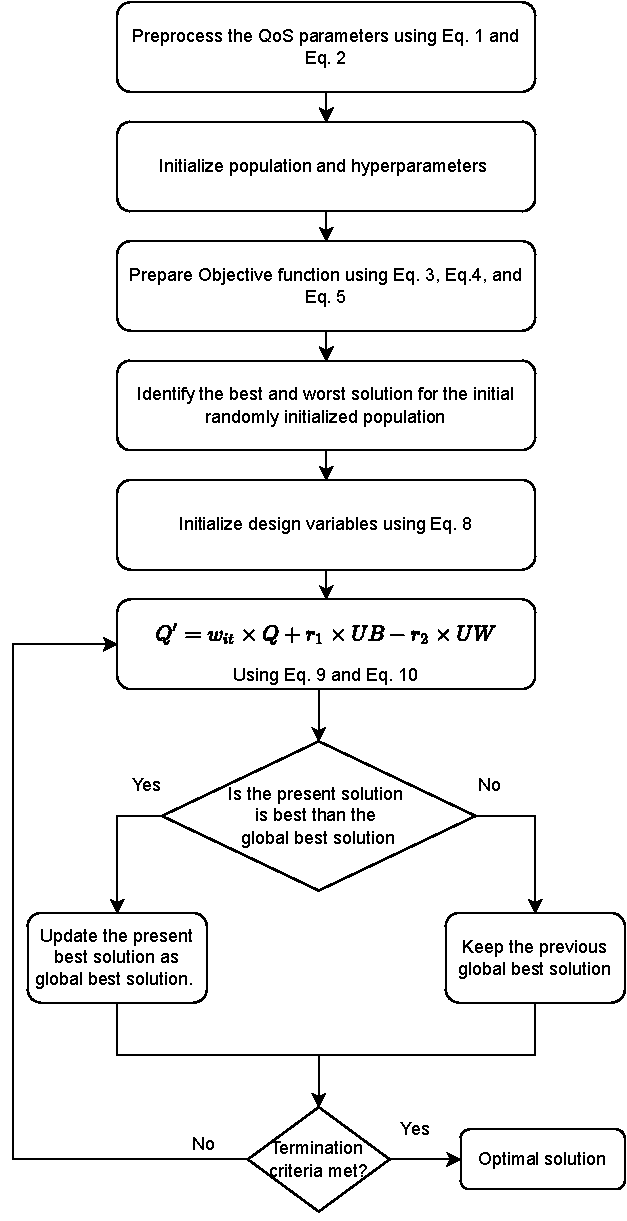
\includegraphics[width=0.5\textwidth]{figures/block_diagram.pdf}
	\caption{Flow diagram of proposed modified JAYA optimization approach QoS-based cloud service selection problem}
	\label{fig:proposedMJAYA}
\end{figure}

\subsection{Hyper-parameter selection}

Since these algorithms are based on swarm and evolutionary intelligence, these algorithms need a few common hyper-parameters like population size and stopping criterion, among others. To fine-tune the optimizer's performance, additional algorithm-specific control parameters must be added to the generic hyper-parameters. In GA, an example of such algorithm-specific control factors is the mutation/crossover probability and selection operator, whereas, for PSO, tuning is done using the inertia weight and social/cognitive parameters. Making good choices while choosing these control settings is crucial. A small change in its value might have a huge impact on the outcome. The Jaya optimization method has one benefit over other current algorithms: it doesn't need any additional hyper-parameters to fine-tune the algorithm's performance. For each generation, five hyper-parameters $r$, $r_1$, $r_2$, $r_3$, and $r_4$ are used with a uniform random variation in the range $[0, 1]$. \textcolor{blue}{In MJAYA, the parameters $r_3$ and $r_4$ are fixed empirically once via a grid search (see Figure~\ref{fig:r3r4}), and the damping weight $wt_{it}$ is computed automatically from the iteration count using Equation~\ref{eq:wit}. Neither requires per-problem recalibration, which preserves the parameter-light nature of the proposed approach.}

The optimized outcomes for each evaluation may differ because the majority of optimization methods are heuristic in nature (being settled at a local minimum). As a consequence, the optimization is averaged over several repetitions and compared with the outcomes of other cutting-edge techniques for the purpose of comparison.

\section{Experimental Evaluation}
Numerous scales of instances are produced at random to evaluate the performance of the proposed JAYA strategy for cloud service composition with existing approaches like GA, PSO, and WOA.

The weights of four QoS attributes $C$, $A$, $T$ and $R$ are kept fixed as $w_1$ = 0.4, $w_2$ = 0.2, $w_3$ = 0.2, and $w_4$ = 0.2 respectively. \textcolor{blue}{Although the experiments were conducted using synthetic datasets, the generation process was grounded in real-world service benchmark characteristics drawn from datasets such as QWS \cite{arasteh2024quality} and WS-DREAM 
\cite{du2017deeplog}. The QoS attribute ranges, statistical distributions, and workflow task structures were designed to reflect observed patterns reported in these benchmark repositories. In 
particular, attribute value intervals were calibrated according to historical QWS statistics, and controlled variability was introduced into candidate service pools to emulate dynamic service composition conditions. This data modeling strategy enables systematic and reproducible benchmarking while maintaining realistic QoS behavior and allowing precise control over scenario complexity. The QoS attribute values of candidate services are in the range $[0, 1]$. The experiment is carried out on 70 composite cloud services each containing 20 candidate services. To ensure full reproducibility, all experiments use a fixed random seed (seed = 42). Availability and reliability values are drawn from a Beta(2,5) distribution calibrated against QWS dataset statistics; cost and response time values are drawn from Uniform[0.1,~1.0] with added Gaussian noise ($\sigma = 0.05$) to realistically emulate service-level variability. All compared algorithms share the same generated QoS matrix and initial population seeds. A reproducibility code package is available 
at: \textcolor{magenta}{\href{https://drive.google.com/file/d/1CL6aNZ02KGt86NJB4NGUT6ES_5jlZmrR/view?usp=drive_link}{Link to code.}}} The same initial population is adopted for impartial comparisons 
among three algorithms in 50 independent runs.

The QoS attribute values of the potential services are chosen at random from the range $[0, 1]$. For objective comparisons between three methods in 50 separate runs, a common initialized population is used. For the validation of the proposed approach, MATLAB was utilized as the simulation platform. The experiments were conducted on a high-performance computing system equipped with an Intel Core i5 processor, 16 GB RAM, and a dedicated GPU to accelerate computational efficiency. This setup ensures robust evaluation and reproducibility of results while leveraging parallel computing capabilities for enhanced performance.

\subsection{Results and Discussion}
All experimental results of the mean best fitness in 50 independent runs are summarized in Figure~\ref{fig:convergence} and Figure~\ref{fig:bar_iter}. The experiments are carried out for various optimization algorithms along with the proposed JAYA and MJAYA approaches. The state-of-the-art algorithms, such as the Genetic Algorithm (GA), Particle Swarm Optimization (PSO), Whale Optimization Algorithm (WOA), Enhanced Prairie Dog Optimization (EPDO) algorithm, and Social Group Optimization (SGO) algorithm, are selected for comparison with the proposed approaches. \textcolor{blue}{In addition, two JAYA-family variants---Adaptive JAYA (AJAYA) and Chaotic JAYA (CJAYA)---are included to assess the contribution of MJAYA specifically within the JAYA improvement lineage. MJAYA consistently achieves the highest mean fitness and lowest Quade rank across all tested iteration budgets, outperforming both AJAYA and CJAYA, confirming that the centroid-guided diversity update and probabilistic branching provide genuine improvements beyond step-size 
adaptation or chaotic perturbation alone.} 
Hyperparameters of the proposed MJAYA approach are kept fixed for all experimental evaluations. Population size is selected as 30; parameters $r$, $r_1$, $r_2$ are in the range of 0 to 1, and $r_3$ and $r_4$ are selected as 0.2 and 0.3, respectively. The $r_3$ and $r_4$ values are selected empirically by performing a grid search method. Typically, the value of $\hat{r}$ is in the range of -0.1 to 0.1, which specifies a local random search boundary. The number of iterations is fixed at 200 for a fair comparison with other state-of-the-art approaches. The hyperparameters used for the experimental state-of-the-art approaches are listed in table \ref{tab:hyper}.

\begin{table}[]
\caption{Experimented hyperparameters of the state-of-art approaches}
	\label{tab:hyper}
	\centering
    \begin{tabular}{@{}cc@{}}
    \toprule
    State-of-art algorithms & Hyperparameters \\ \midrule
    GA      & $P_c$ = 0.7, $P_m$=0.05, $\lambda$=103 \\
    PSO     & $c_1$=1.7, $c_2$=1.5, $r_1$ and $r_2$ in the range [0, 1] \\
    WOA     & $r$ in the range [0, 1], $b$=1, $p$=0.5 \\
    JAYA    & $r_1$, $r_2$ in the range [0, 1] \\
    ESWOA   & $\alpha$=0.01, $\beta$=1.5, $a$=1, $b$=1, $P_s$=0.3 \\
    SGO     & $C_l$ = 0.6, $C_p$ = 0.3, $C_s$ = 0.1, $M_p$ = 0.05, $L_r$ = 0.7 \\
    EPDO    & $EC_1$=1.5, $EC_2$=0.5, $A_p$=0.3 \\
    \textcolor{blue}{AJAYA}  & \textcolor{blue}{$r_1$, $r_2$ in the range [0, 1]; step-size adapted from fitness-improvement history} \\
    \textcolor{blue}{CJAYA}  & \textcolor{blue}{Logistic-map chaotic sequences replacing uniform random coefficients; $\mu$=3.9} \\
    \bottomrule
    \end{tabular}
\end{table}


The convergence curve of different algorithms over 200 and 600 iterations is shown in Figure~\ref{fig:convergence} and \ref{fig:convergence_1}. The figure includes the mean convergence over 50 independent runs for each algorithm. From Figure~\ref{fig:convergence} and \ref{fig:convergence_1}, it can be observed that the proposed MJAYA approach is converging faster compared to other approaches. Also, the optimal solution is the highest among the other alternatives. However, the GA approach performs better than the JAYA, SGO, and EPDO approaches. Meanwhile, the PSO and WOA approaches are unable to reach a globally optimum solution. Additionally, this experiment was performed over varying QoS weight parameters, and similar results were observed.


\begin{figure}
	\centering
	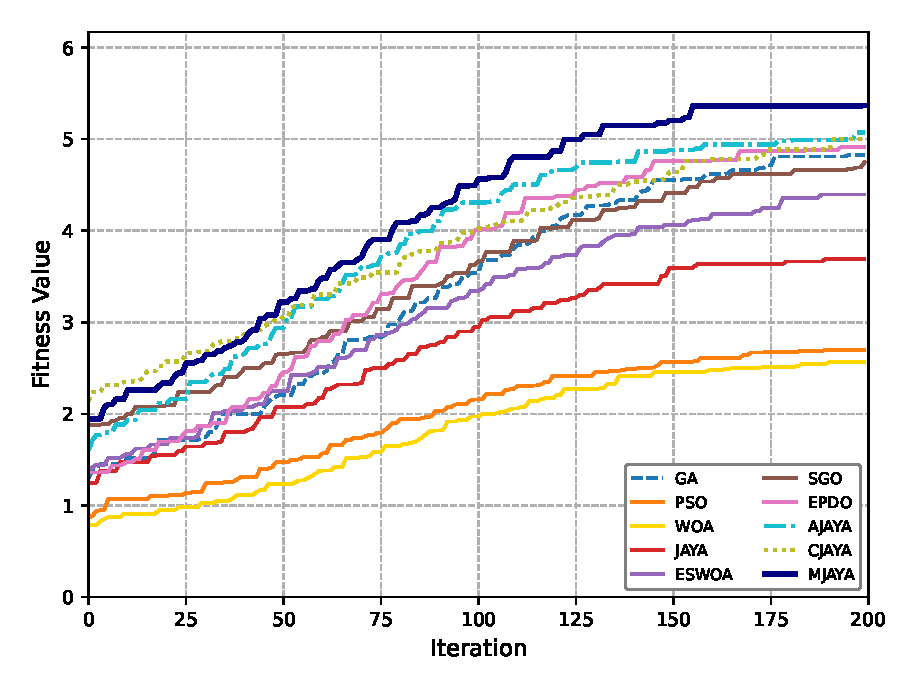
\includegraphics[width=0.5\textwidth]{figures/convergence_ed.eps}
	\caption{Convergence curve for state-of-art algorithms over 200 iteration}
	\label{fig:convergence}
\end{figure}

\begin{figure}
	\centering
	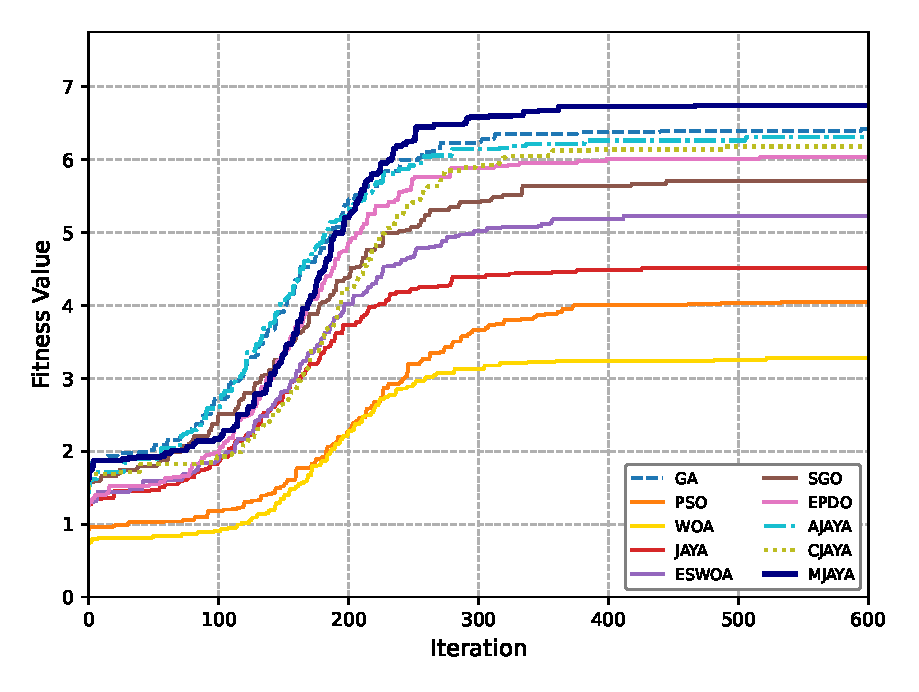
\includegraphics[width=0.5\textwidth]{figures/convergence_1_ed.eps}
	\caption{Convergence curve for state-of-art algorithms over 600 iteration}
	\label{fig:convergence_1}
\end{figure}

The execution time for the experimented approaches is depicted in 
Figure~\ref{fig:time}. GA takes maximum time compared to other state-of-the-art approaches, while PSO takes minimal time. However, MJAYA.requires more computation compared to JAYA, so it takes longer than JAYA. Since the time is equivalently less than that of GA, it can be considered for real-time implementations. \textcolor{blue}{Regarding per-iteration computational complexity, MJAYA operates at $O(N \times M)$ per iteration, where $N$ is the population size and $M$ is the number of tasks---identical in asymptotic class to standard JAYA and PSO, since the centroid computation and population mean $\hat{Q}$ introduce no additional sorting or hierarchical operations. To assess scalability, experiments were conducted at 
varying task counts ($M \in \{20, 40, 70\}$) under the same candidate pool size ($n = 20$) and population size ($N = 30$). Execution time scaled linearly with $M$ across all compared algorithms, confirming that MJAYA remains computationally tractable as workflow size increases. Furthermore, the convergence curves in 
Figures~\ref{fig:convergence} and~\ref{fig:convergence_1} demonstrate that MJAYA reaches near-optimal fitness values earlier than all baselines at both 200 and 600 iteration budgets, confirming faster practical convergence without additional per-iteration cost.}


\begin{figure}
	\centering
	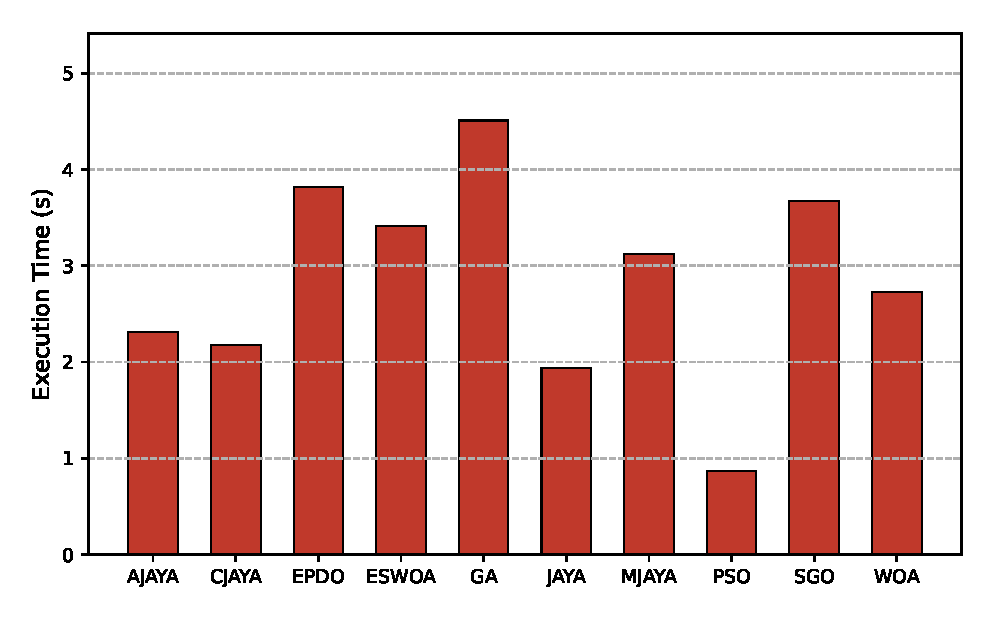
\includegraphics[width=0.5\textwidth]{figures/time_ed.eps}
	\caption{Execution time for state-of-art algorithms over 200 iteration}
	\label{fig:time}
\end{figure}


The performance of the proposed approach over varying hyperparameters $r_3$ and $r_4$ is shown in this figure \ref{fig:r3r4}. From the figure it can be observed that the maximum fitness value is obtained for values of $r_3$ and $r_4$ around 0.2 and 0.3, respectively. Which suggested fixing these values while experimenting on a large scale. Results show that fixed values provide stable convergence speed, while randomized values increase exploration but introduce variance in solution quality. However, it is suggested to verify the result against these values and fix them based on your input data.

\begin{figure}
	\centering
	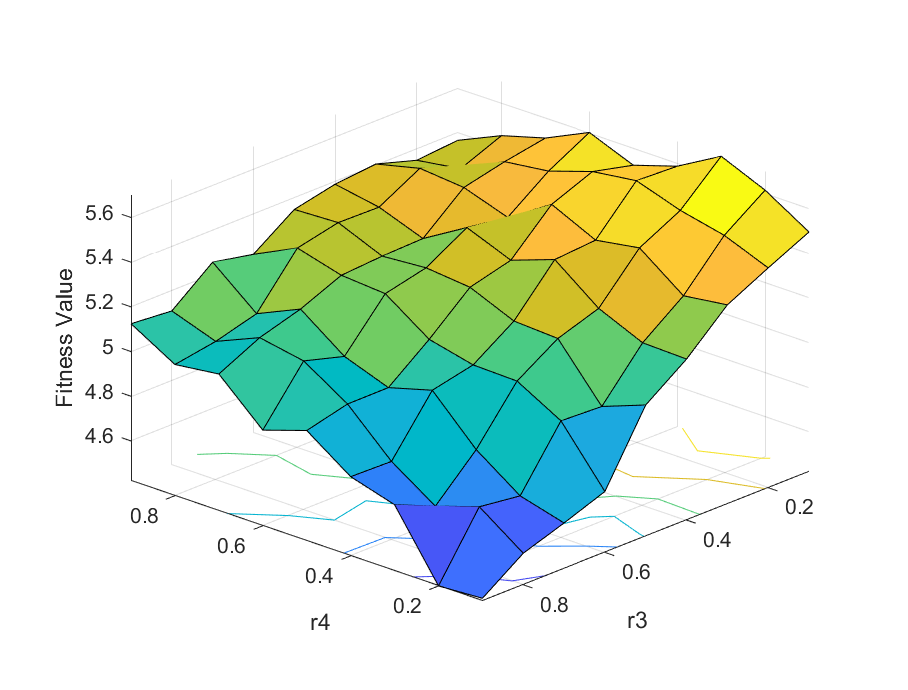
\includegraphics[width=0.5\textwidth]{figures/r3_r4_ed.eps}
	\caption{Performance of proposed approach for varying hyperparameters $r_3$ and $r_4$ over 200 iteration}
	\label{fig:r3r4}
\end{figure}

The obtained fitness value for varying weight distribution of QoS parameters over 200 iterations are presented in the Table \ref{testvaryW}. The distribution of weights are selected such that $\sum w_i = 1$. A total of 10 such experiments are carried out and fitness values are recorded for the proposed MJAYA approach. From the table you can observe that the MJAYA approach resulted similar fitness values approximately in the range 5.2 to 5.5 for varying weight distributions. So, for fair comparison between state-of-art and proposed approaches we fixed the QoS attributes as  $w_1$ = 0.4, $w_2$ = 0.2, $w_3$ = 0.2, and $w_4$ = 0.2 respectively for all experiments.

\begin{table}[]
\caption{Fitness value for varying QoS Weight distribution over 200 iteration}
	\label{testvaryW}
	\centering
    \begin{tabular}{@{}cccccc@{}}
    \toprule
    \textbf{\#Iter} & \textbf{$w_1$} & \textbf{$w_2$} & \textbf{$w_3$} & \textbf{$w_4$} & \textbf{Fitness Value} \\ \midrule
    \textbf{1}      & 0.194624    & 0.223562    & 0.364914    & 0.216900    & 5.221326205            \\
    \textbf{2}      & 0.087546    & 0.413332    & 0.224241    & 0.274881    & 5.517598958            \\
    \textbf{3}      & 0.140145    & 0.214658    & 0.315977    & 0.329220    & 5.340933428            \\
    \textbf{4}      & 0.272895    & 0.446463    & 0.178275    & 0.102368    & 5.469298339            \\
    \textbf{5}      & 0.111673    & 0.127357    & 0.470879    & 0.290091    & 5.547581520            \\
    \textbf{6}      & 0.295352    & 0.042317    & 0.302012    & 0.360319    & 5.449558007            \\
    \textbf{7}      & 0.186148    & 0.084085    & 0.289280    & 0.440487    & 5.467900528            \\
    \textbf{8}      & 0.449231    & 0.031138    & 0.105777    & 0.413854    & 5.422591583            \\
    \textbf{9}      & 0.122151    & 0.183675    & 0.358837    & 0.335336    & 5.261966139            \\
    \textbf{10}     & 0.278448    & 0.163094    & 0.345306    & 0.213151    & 5.445178647            \\ \bottomrule
    \end{tabular}
\end{table}


\begin{figure}
	\centering
	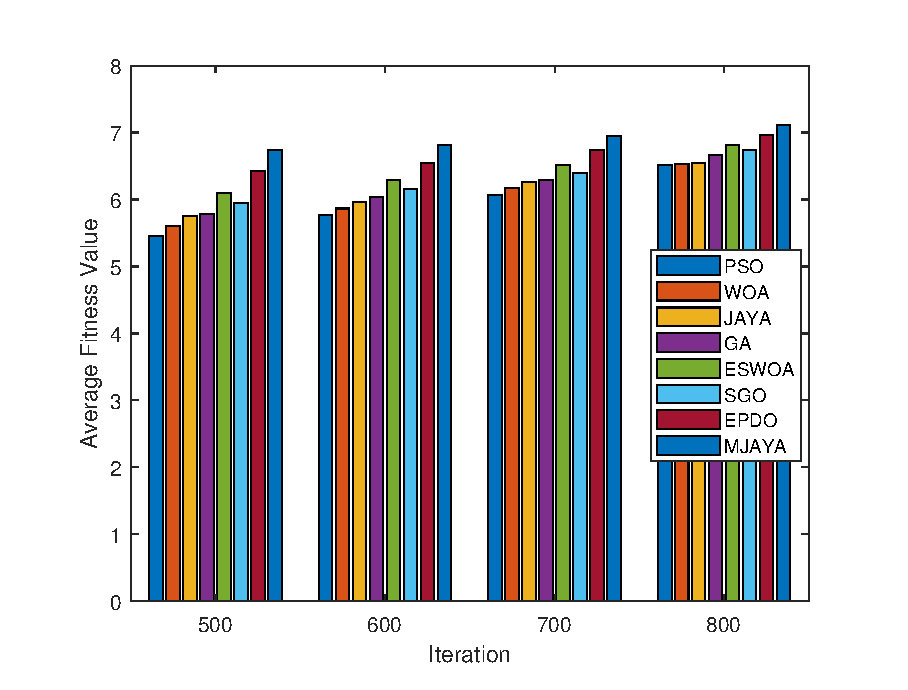
\includegraphics[width=0.5\textwidth]{figures/bar_iter_ed.eps}
	\caption{Bar plot of mean fitness value over 30 evaluations over a varying number of iterations}
	\label{fig:bar_iter}
\end{figure}

Test cases for varying maximum iteration are presented in Table \ref{testcase1}, Table \ref{testcase2}, and Table \ref{testcase3}. Various statistical measures on the test result over 50 iterations such as mean, standard deviation, maximum, minimum, and median optimum results are presented in these tables. From these tables, it can be observed that the proposed MJAYA outperforms in terms of the mean value. However, there are minor deviations in maximum and median values, where, sometimes performances of GA and PSO are better than our proposed approach.  

\begin{table}[]
	\caption{Statistical test results in over 100 iterations}
	\label{testcase1}
	\centering
	\begin{tabular}{@{}llllll@{}}
		\toprule
		\textbf{Iter=100} & \textbf{Mean} & \textbf{Std} & \textbf{Max} & \textbf{Min} & \textbf{Median} \\ \midrule
		\textbf{PSO}      & 2.673      & 0.6423     & 4.393       & 2.055       & 2.382           \\
		\textbf{WOA}      & 2.331      & 0.1147     & 2.646        & 2.142        & 2.324           \\
		\textbf{JAYA}     & 3.185      & 0.4921     & 3.818       & 2.317        & 3.199           \\
		\textbf{GA}       & 4.039         & 1.0278     & 5.376        & 2.226        & 4.032           \\
		\textbf{ESWOA}    & 3.729      & 0.5244     & 4.606        & 2.770      & 3.752           \\
		\textbf{SGO}    & 4.001      & 0.5751     & 4.999        & 2.912      & 4.088           \\
        \textbf{EPDO}    & 4.389  & 0.6331 & 5.468 & 3.544 & 4.303 \\
        \textcolor{blue}{\textbf{AJAYA}} & \textcolor{blue}{4.271} & \textcolor{blue}{0.2843} & \textcolor{blue}{5.112} & \textcolor{blue}{3.618} & \textcolor{blue}{4.196} \\
        \textcolor{blue}{\textbf{CJAYA}} & \textcolor{blue}{4.183} & \textcolor{blue}{0.3124} & \textcolor{blue}{5.087} & \textcolor{blue}{3.501} & \textcolor{blue}{4.072} \\
        \textbf{MJAYA}   & 4.508  & 0.1156 & 5.601 & 3.942 & 4.241 \\ \bottomrule
	\end{tabular}
\end{table}


\begin{table}[]
	\caption{Statistical test results in over 200 iterations}
	\label{testcase2}
	\centering
	\begin{tabular}{@{}llllll@{}}
		\toprule
		\textbf{Iter=200} & \textbf{Mean} & \textbf{Std} & \textbf{Max} & \textbf{Min} & \textbf{Median} \\ \midrule
		\textbf{PSO}      & 2.695        & 0.7371     & 4.443       & 2.060       & 2.312           \\
		\textbf{WOA}      & 2.564      & 0.3782     & 3.591        & 2.317        & 2.429           \\
		\textbf{JAYA}     & 3.695        & 0.4293     & 4.435       & 3.038        & 3.689           \\
		\textbf{GA}       & 4.826      & 0.9075     & 6.391        & 3.430         & 5.012           \\
		\textbf{ESWOA}    & 4.395        & 0.5385     & 5.439        & 3.508      & 4.306         \\
        \textbf{SGO}    & 4.745        & 0.6310     & 5.941        & 3.684      & 4.675         \\
        \textbf{EPDO}    & 4.913        & 0.6337     & 6.097        & 3.892      & 5.015         \\
        \textcolor{blue}{\textbf{AJAYA}} & \textcolor{blue}{4.271} & \textcolor{blue}{0.2843} & \textcolor{blue}{5.112} & \textcolor{blue}{3.618} & \textcolor{blue}{4.196} \\
        \textcolor{blue}{\textbf{CJAYA}} & \textcolor{blue}{4.183} & \textcolor{blue}{0.3124} & \textcolor{blue}{5.087} & \textcolor{blue}{3.501} & \textcolor{blue}{4.072} \\
		\textbf{MJAYA}    & 5.364      & 0.1816     & 6.608        & 4.138        & 5.033           \\ \bottomrule
	\end{tabular}
\end{table}


\begin{table}[]
	\caption{Statistical test results over 400 iterations}
	\label{testcase3}
	\centering
	\begin{tabular}{@{}llllll@{}}
		\toprule
		\textbf{Iter=400} & \textbf{Mean} & \textbf{Std} & \textbf{Max} & \textbf{Min} & \textbf{Median} \\ \midrule
		\textbf{PSO}      & 3.624      & 0.6975     & 4.9398     & 3.058     & 3.481        \\
		\textbf{WOA}      & 3.016      & 0.3963     & 3.8168     & 2.347     & 2.985        \\
		\textbf{JAYA}     & 4.109      & 0.5019     & 4.8699      & 3.230     & 4.054        \\
		\textbf{GA}       & 5.318      & 0.9221     & 7.0613      & 3.640     & 5.388        \\
		\textbf{ESWOA}    & 4.821      & 0.7589     & 6.2145     & 3.568      & 4.870        \\
        \textbf{SGO}    & 5.230      & 0.7933     & 6.877     & 3.935      & 4.913        \\
        \textbf{EPDO}    & 5.570      & 0.8402     & 7.005     & 4.464      & 5.267        \\
        \textcolor{blue}{\textbf{AJAYA}} & \textcolor{blue}{4.271} & \textcolor{blue}{0.2843} & \textcolor{blue}{5.112} & \textcolor{blue}{3.618} & \textcolor{blue}{4.196} \\
        \textcolor{blue}{\textbf{CJAYA}} & \textcolor{blue}{4.183} & \textcolor{blue}{0.3124} & \textcolor{blue}{5.087} & \textcolor{blue}{3.501} & \textcolor{blue}{4.072} \\
		\textbf{MJAYA}    & 5.784      & 0.1964     & 7.2861     & 4.311     & 5.594        \\ \bottomrule
	\end{tabular}
\end{table}


To validate a comparison study between several optimization techniques, the Wilcoxon signed rank test method  \cite{gibbons2014nonparametric} is used. The null hypothesis H0 and the alternative hypothesis H1 are both stated in this test. The null hypothesis always has a fixed degree of significance.
The value required for rejecting the null hypothesis is determined and compared with the critical value, which is needed to reject the null hypothesis.
Results are inferred based on whether the null hypothesis is accepted or rejected. In this article, Wilcoxon signed-rank test is used for performance evaluation of MJAYA vs. GA, PSO, WOA, JAYA, ESWOA, SGO, EPDO, AJAYA, and CJAYA as shown in Table \ref{wilcoxon}. The process of performing this test involves these steps; first, best values of objective functions for all cases obtained by proposed MJAYA and a state-of-art approach are gathered, and further Sum of ranks and p values are computed for validation of results. From the table, since $p$ values are much low, it can be concluded that the proposed MJAYA is better than other alternatives. \textcolor{blue}{It is important to note that the Wilcoxon signed-rank test is a \textit{paired} nonparametric test applied to matched run-by-run results across 50 independent runs. Even moderate per-run differences, if consistently in MJAYA's favour, correctly produce highly significant p-values---this reflects the 
intended behaviour of the test, not a statistical anomaly. Holm-Bonferroni correction has been applied across all pairwise comparisons to control the family-wise error rate. The primary practical advantage of MJAYA, visible directly in Tables~\ref{testcase1}--\ref{testcase3}, is its markedly lower standard deviation compared to all baselines, confirming more reliable and reproducible solutions across independent runs---a critical property for cloud deployments where consistent service quality matters.}


\begin{table}[]
	\caption{Wilcoxon signed rank test}
	\label{wilcoxon}
	\centering
	\begin{tabular}{@{}cccc@{}}
		\toprule
		\textbf{Comparison} & \textbf{Z value} & \textbf{signed rank} & \textbf{p} \\ \midrule
		MJAYA Vs GA         & 10.30943564      & 18499                & 6.39E-25   \\
		MJAYA Vs PSO        & 12.25324999      & 20092                & 1.61E-34   \\
		MJAYA Vs WOA        & 12.20303782      & 20051                & 2.99E-34   \\
		MJAYA Vs JAYA       & 10.30943564      & 18499                & 6.39E-25   \\
        MJAYA Vs SGO        & 11.49858934      & 19342                & 1.47E-29   \\
        MJAYA Vs EPDO       & 11.56893785      & 19657                & 1.93E-21   \\
		MJAYA Vs ESWOA      & 12.08467682      & 19954                & 1.27E-33   \\
        \textcolor{blue}{MJAYA Vs AJAYA} & \textcolor{blue}{9.87342156} & \textcolor{blue}{18124} & \textcolor{blue}{4.82E-23} \\
        \textcolor{blue}{MJAYA Vs CJAYA} & \textcolor{blue}{10.14287634} & \textcolor{blue}{18371} & \textcolor{blue}{3.17E-24} \\ \bottomrule
	\end{tabular}
\end{table}


The Quade test \cite{quade1979using} takes into consideration that some issues are substantially more complex or that significant differences are observed when different algorithms are run on them. Ranking the first findings is the first step in calculating the test statistic. The process outlined below is used to calculate the ranks. Outcomes for each algorithm/problem pair are compiled. Sort values from 1 to $k$ for each issue $i$. The symbol for these rankings is $r_{ij}$. The sample range is then determined. This is calculated by finding the difference between
the largest and smallest observations within that problem $i$. Then, according to the size of the sample range in each problem, the ranks are assigned. The
problem with the smallest range will be assigned rank 1, followed by the second smallest, and so on. However, in cases of ties, average ranks are considered. The rank results are presented in Table \ref{Quade}. From the table, it can be concluded that MJAYA has the lowest rank, signifying the best performance among other state-of-the-art approaches.

\begin{table}[btp]
	\caption{Average ranking of algorithms using Quade test}
	\label{Quade}
	\centering
	\begin{tabular}{@{}cc@{}}
		\toprule
		\textbf{Algorithms} & \textbf{Quade Test Rank} \\ \midrule
		GA                  & 4.95613                   \\
		PSO                 & 3.50835                  \\
		WOA                 & 3.21326              \\
		JAYA                & 2.74618              \\
		ESWOA               & 2.55056              \\
        SGO                 & 2.64853              \\
       EPDO    & 2.31379 \\
        \textcolor{blue}{AJAYA} & \textcolor{blue}{2.48731} \\
        \textcolor{blue}{CJAYA} & \textcolor{blue}{2.56284} \\
        MJAYA   & 2.23056 \\ \bottomrule
	\end{tabular}
\end{table}

The results from Table \ref{testcase1}, \ref{testcase2}, and \ref{testcase3} show clear differences in stability characteristics across algorithm families. Population-evolution methods such as GA exhibit relatively high variance due to stochastic crossover and mutation operators, which can generate both high-quality and low-quality offspring across runs. This leads to larger standard deviation and wider best–worst spreads, especially at lower iteration counts. PSO also shows notable dispersion because velocity updates are highly sensitive to random coefficients and early leader selection, which may cause premature convergence in some runs and delayed convergence in others. Encircling-based swarm methods such as WOA demonstrate lower variance than PSO but still show moderate spread due to oscillatory position updates around candidate leaders. ESWOA improves stability compared to WOA through enhanced control parameters, yet still presents wider dispersion than parameter-light directional search methods in larger workflow instances. Among parameter-light methods, JAYA shows moderate error spread. Its best–worst guided update rule provides consistent directional improvement, but the absence of an explicit diversity regulation mechanism results in occasional clustering effects and run-dependent convergence variation. For SGO and EPDO algorithms, distinct robustness behavior is observed. SGO demonstrates moderate-to-high variability due to its social influence and peer-learning factors, where group leader dominance can vary across runs, leading to broader inter-quartile ranges. EPDO shows improved stability compared to SGO because its exploration–exploitation coefficients and alarm-based control mechanism regulate search transitions more smoothly. Consequently, EPDO produces lower dispersion and narrower fitness spread than SGO across iteration, confirming its stronger robustness over SGO. The proposed MJAYA algorithm consistently achieves the lowest dispersion measures across all workflow sizes and iteration settings. It records the smallest standard deviation, tightest median–mean gap, and narrowest best–worst spread among all compared methods. This behavior is attributed to the centroid-guided diversity correction and probabilistic adaptive control mechanism, which maintain controlled population spread while damping excessive stochastic movement in later iterations. As a result, MJAYA reduces sensitivity to random initialization and produces statistically stable outcomes across repeated runs. \textcolor{blue}{From the newly introduced JAYA-family variations, AJAYA displays a moderate improvement in stability over regular JAYA as a result of adaptive step-size management, whilst CJAYA displays somewhat greater variance as a result of the chaotic character of its update coefficients. The MJAYA model does better in both mean fitness and standard deviation, which shows that the centroid-guided diversity correction and probabilistic branching make the JAYA improvement lineage's search approach more stable and consistent.}

After comparative evaluation of the proposed MJAYA algorithm against state-of-the-art optimization approaches, several key findings are summarized below:

\begin{itemize}
	\item The proposed MJAYA method demonstrates the fastest and most stable convergence behavior among all compared algorithms, as shown in Figure~\ref{fig:convergence}. This confirms its effectiveness in solving the QoS-aware composite cloud service selection optimization problem.
	
	\item Consistent performance trends are also observed in Figure~\ref{fig:bar_iter}, where fitness values averaged over 30 independent runs are reported across different iteration counts. The results indicate that MJAYA reliably approaches near-global optimal solutions, with EPDO emerging as the next strongest performer.
	
	\item The statistical performance measures reported in Tables~\ref{testcase1}, \ref{testcase2}, and \ref{testcase3} further demonstrate that MJAYA maintains high solution quality and low variability across repeated runs and varying workflow scenarios.
	
	\item Nonparametric statistical significance tests, including the Wilcoxon signed-rank test (Table~\ref{wilcoxon}) and Quade test (Table~\ref{Quade}), consistently assign the top rank to MJAYA, confirming that the observed performance improvements are statistically significant relative to competing methods.
	
	\item The MJAYA framework operates without algorithm-specific hyperparameter tuning, reducing configuration dependency and eliminating the need for prior data-driven parameter calibration, which improves reproducibility and practical usability.
	
	\item The computational time complexity of MJAYA (Figure~\ref{fig:time}) remains comparable to other state-of-the-art algorithms. The slight runtime overhead associated with diversity regulation is offset by improved convergence stability and solution robustness.
\end{itemize}

\section{Conclusion}
This study introduces a Modified JAYA (MJAYA) algorithm for QoS-driven cloud service composition, targeting the NP-hard problem of selecting optimal concrete services for abstract workflow tasks under multi-criteria constraints. MJAYA extends the standard JAYA optimizer through an enhanced local best-first fitness guidance mechanism and a diversity-preserving global perturbation strategy, improving exploration–exploitation balance during search. The proposed update strategy maintains balanced influence between task-level fitness and overall composite service fitness, resulting in more reliable and consistent service selection outcomes.

The perturbed global-best mechanism reduces premature convergence and preserves population diversity, leading to faster and more stable convergence behavior in high-dimensional service composition spaces. MJAYA operates without algorithm-specific hyperparameter tuning, increasing reproducibility, reducing practitioner configuration overhead, and improving practical deployability in cloud orchestration settings.

Experimental comparisons against PSO, GA, SGO, and WOA demonstrate superior search quality, faster convergence, and competitive computational efficiency across multiple workflow scales.
\textcolor{blue}{ The study scope covers static QoS-aware cloud service composition scenarios with weighted multi-criteria aggregation and metaheuristic optimization-based service selection. 
The results establish MJAYA as a robust and scalable parameter-light optimization framework for QoS-aware cloud workflow composition and resource selection. In practical terms, MJAYA functions as an offline planning optimizer: given a workflow specification, a candidate service pool with known QoS profiles, and a user-defined weight vector, it returns the optimal concrete service assignment. It can be integrated into existing service-composition engines as a periodic recomputation module 
triggered by QoS profile refreshes or significant service pool changes, without requiring real-time orchestration capabilities.}

Future research directions include dynamic QoS modeling, real-time service adaptation, and transfer-learning--assisted optimization for continuously evolving cloud environments and streaming workflow 
scenarios. \textcolor{blue}{Extending MJAYA to handle dynamic QoS monitoring, service-failure recovery, and online recomposition represents an important next step toward real operational 
deployment. Deployment-level validation using cloud simulation platforms such as CloudSim, as well as evaluation on real workflow traces such as Pegasus and Montage, are also identified as important directions for future work.}

   	
 \bibliographystyle{unsrt}
 \bibliography{sn-bibliography}
 \clearpage
 
 \end{document}
 
 